\justifying
\NSFCBodyText

\subsubsection{与本项目相关的研究工作积累}
申请人颜丰为新疆大学副教授、博士、硕士研究生导师，已开展多模态视觉表征、特征交互及深度学习模型研究。相关工作能够支撑双时相影像的表征建模、方法对照与训练评测，但已有任务与矿山变化检测的标签和目标不同，需要通过专门实验验证迁移效果。

在跨模态检索研究中，申请人作为通讯作者参与Feature Fusion Mamba Hashing via Decoupling方法的研究构思、方法设计、实验指导、结果分析及论文修改\cite{Tang2026Hashing}。该积累与本项目中的表征分离和受控消融有关，可用于组织变化与背景特征分析，不能直接作为矿山域泛化已经有效的证据。

在遥感视觉问答研究中，RSHR+工作涉及问题条件下的视觉校准和结构化状态空间推理，申请人作为通讯作者承担研究构思、方法设计、实验指导及写作工作\cite{Xu2026RSHR}。这一经历支持遥感影像表征与实验执行能力；其中“视觉校准”指任务相关的表征处理，与本课题的概率校准概念不同，既有结果不能替代本课题的可靠性验证。

\subsubsection{已取得的研究工作成绩}
代表性成果还包括Knowledge-Aware Image Understanding with Multi-Level Visual Representation Enhancement，发表于\textit{Machine Learning}，申请人为第一作者及通讯作者，负责研究构思、方法设计、实验指导、分析与写作\cite{Yan2024Knowledge}。上述成果的题录及贡献已由申请人事实资料确认，支撑从问题定义到模型比较和结果分析的科研执行能力。RSHR+已有正式DOI及卷期题录，本稿不将未来印刷卷期表述为已经完成纸本出版，正式申报时以出版页面状态为准。

\textbf{公开数据预实验（MCT-P01）。}2026年9月6日，基于MineNetCD作者发布的256像素裁切数据完成了三组对照\cite{Yu2024MineNetCD}。训练、验证四个分片均通过SHA256校验；按矿区及行号的固定哈希抽取50个训练矿区的1,188对影像和10个验证矿区的480对影像，矿区ID及完全重复影像对不交叉。采用118,593参数的轻量孪生网络，对无一致性约束、全区域约束、背景位置约束分别运行种子17、29、43；每组固定12轮、阈值0.5。同种子保持初始化、批次及增强一致，背景掩码只用于训练。九个末轮模型全部保存后统一评分，未按验证性能调参或选模型。

预实验执行流程见图\ref{fig:mct-pilot-workflow}。
\begin{figure}[!htbp]
  \centering
  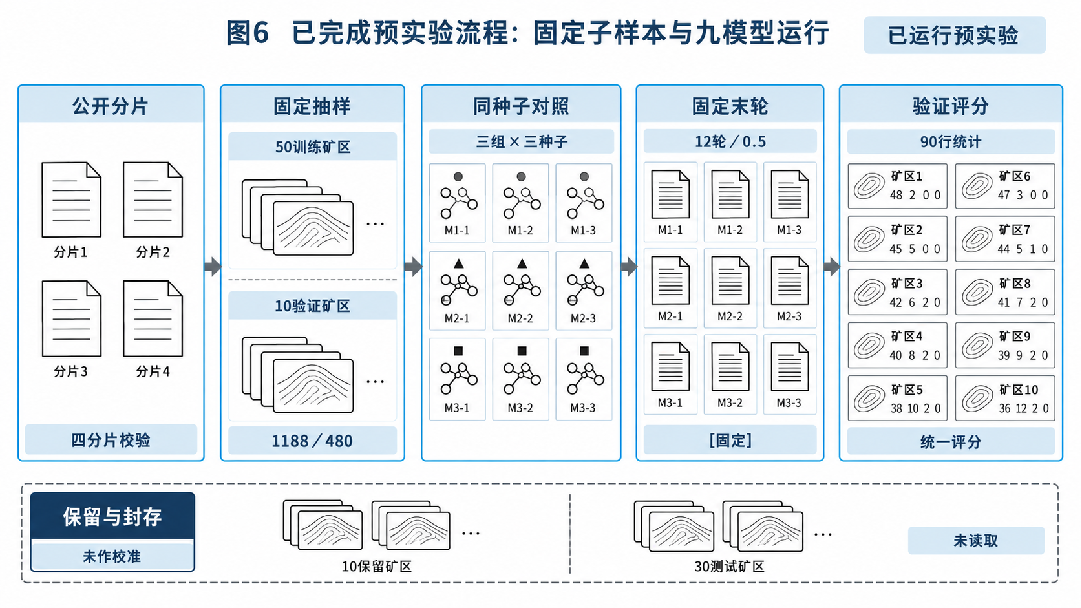
\includegraphics[width=\linewidth,trim=0 0 0 12mm,clip]{figures/F14_pilot_workflow.pdf}
  \captionsetup{justification=justified,singlelinecheck=false}
  \caption{已完成预实验流程。固定抽取1,188对训练影像和480对验证影像，运行三组各三个种子后统一评分。右侧矿区卡片及其数字仅示意汇总方式，不作为实测统计；真实结果见图\ref{fig:mct-pilot-results}。10个保留矿区未作校准，30个官方测试矿区未读取。}
  \label{fig:mct-pilot-workflow}
\end{figure}

每矿区先汇总像素计数，再等权平均；下表为三个种子的均值，单位为百分数。完整种子离散程度、90行矿区计数和权重哈希已归档，三组比较与矿区配对效应见图\ref{fig:mct-pilot-results}。
\begin{center}
\begin{tabular}{lrrr}
\hline
训练约束 & 变化IoU & 背景误报率 & 总体召回率 \\
\hline
无一致性约束 & 21.08 & 24.13 & 67.82 \\
全区域约束 & 20.96 & 26.62 & 72.65 \\
背景位置约束 & 21.72 & 23.28 & 68.55 \\
\hline
\end{tabular}
\end{center}

按矿区内先平均种子、再配对bootstrap 10,000次计算探索性95\%区间。背景相对全区域的IoU差为$+0.76$个百分点，区间$[-0.06,1.52]$跨零；背景误报率差为$-3.35$个百分点，区间$[-4.22,-2.57]$，同时总体召回差为$-4.11$个百分点，区间$[-6.24,-2.23]$。降误报伴随召回下降；相对无约束的IoU和误报率差区间也跨零。预先定义的片内、不接边且面积不超过64像素的8连通变化区在验证子样本中为零，小变化召回不可估计，未事后改变阈值。

\begin{figure}[!htbp]
  \centering
  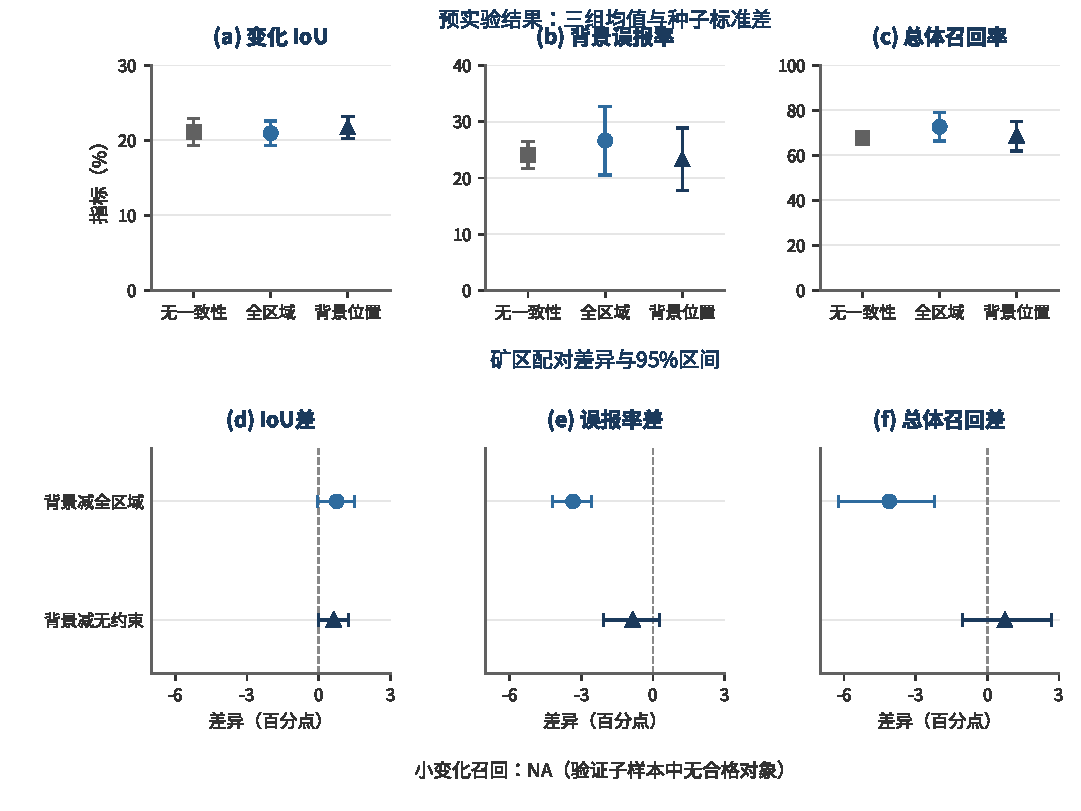
\includegraphics[width=\linewidth]{figures/F15_F16_pilot_results.pdf}
  \captionsetup{justification=justified,singlelinecheck=false}
  \caption{预实验结果与矿区配对效应。上排为三个种子的矿区宏平均及种子样本标准差，单位为\%；下排先在矿区内平均种子，再对10个矿区配对重采样，展示差值及95\%区间，单位为百分点。背景相对全区域的降误报伴随总体召回下降；相对无约束的三项区间均跨零，小变化召回为NA。}
  \label{fig:mct-pilot-results}
\end{figure}

该预实验提供了可复现的矿山数据运行及误差证据，但尚不支持“降误报并保持细小变化检出”的联合假说。当前仅约束背景位置，深层特征仍可能感受邻近变化区；相同权重也不保证实际梯度强度相同。后续需核验原始场景的小变化端点，完成强近邻、随机掩码和强度匹配对照。完整版归档、官方测试和可靠性实验尚未完成。

\textbf{外观差异代理量的可计算性与混杂（MCT-P01-EXT-Ds）。}在同一批480个验证切片上计算了本申请所定义的外观差异代理量$D_s$，归一化与腐蚀口径与上述预实验一致，逐样本哈希全部校验通过；该扩展不训练模型，误差数值取自上表所依据的逐矿区结果，官方测试矿区同样未读取。474对可计算$D_s$，6对因腐蚀后无有效未变化像素记为不适用，矿区级$D_s$跨度0.0915—0.2196。按矿区$D_s$中位数分档，三组约束下高档的背景误报率均高于低档（背景组19.07\%对27.49\%），方向符合预期，但置换检验p值在0.28—0.57之间，10个矿区不足以支持确认性结论。

需要在正式方案中处理的是一处混杂：高$D_s$档的变化IoU同样更高（背景组17.83\%对25.61\%），与“外观差异使任务更难”的朴素预期相反。检查发现$D_s$与矿区变化像素占比同向共变（Spearman $+0.370$，置换p=0.295），低档矿区平均变化像素占比7.24\%、高档13.06\%。变化像素占比直接影响IoU的分母结构，因此按$D_s$分层的组间差异不能单独归因于外观差异。正式实验按$D_s$分层时将同时报告各档的变化像素占比，分层结论以背景误报率为主，不用变化IoU解释外观差异的作用。

\FloatBarrier
\subsubsection{可行性分析}
本课题所需的核心能力是影像表征建模、训练协议管理、对照实验与误差分析，申请人的已有工作为这些环节提供了方法基础。任务采用公开数据和可复现基线，先固定单一骨干分析约束区域，再冻结检测器评价可靠性，能够减少同时改动多个环节带来的实验成本。

申请人负责科学问题凝练、方法设计和结果审查。数据追溯、模型复现、统计评测的实际承担人员与投入计划为\textbf{【待补 F-MCT-01：本课题成员、分工与投入时间】}。矿山标签解释、案例抽查及实验室合作由\textbf{【待补 F-MCT-02：专业合作者与已确认的协作事项】}落实。启动时优先完成主数据与同骨干对照；专业协作未落实前，研究解释限定在影像变化标签层面。

\subsubsection{研究风险与应对措施}
\textbf{数据与语义风险。}若归档元数据不能追溯矿区和原始场景，暂停未见矿区泛化结论，向发布者核实来源或改用有明确来源的分组实验。若配准和标签争议主导误差，先记录质量问题和敏感性结果，收窄可解释样本范围，剔除规则不得依赖测试性能。

\textbf{机制与效果风险。}若背景约束只重复已有方法、或小变化召回受到实质损伤，停止把该约束作为优势方法，保留负迁移边界及反例分析。若误差排序与简单熵无明显差异，报告其无增量范围，不继续叠加复杂可信模块。结论依据预定对照与矿区效应区间，并保留失败案例。

\textbf{实施与产出风险。}非独占算力、人员投入和论文审稿时间均会影响进度。先测量单配置耗时，据实际资源排期冻结核心实验，优先保留强近邻与关键消融，缩减外部数据扩展。论文写作与核心实验同步推进，为修改及发表留出时间；中期和结题节点按实验室安排执行，不能以投稿替代指南要求的源刊论文发表。
